% Tech Stack and Standards:
% List the likely tech stack for your application (distinguish between back-end and front-end, programming languages and frameworks)
% Agree on tools for communication and development (e.g., Slack, IDEs, etc.)
% Agree on coding standards
% Provide justifications for your choices

\section{Tech Stack and Standards}
\begin{spacing}{1.3}

\subsection{Team Communications}
\paragraph{Technologies Considered:}
Slack, Facebook Messenger, Email, Discord

\paragraph{Decision Criteria:}
\begin{itemize}
\item Instant messaging
\item Multiple text channels
\item Voice channel support
\item GitHub integration
\item Currently used services
\end{itemize}

\paragraph{Chosen:}
Discord

\paragraph{Justification:}
Slack and Discord rated highest for instant messaging, text channel support and reliable voice channel service. Despite Slack having better integration capabilities with GitHub, Discord was chosen as it was already regularly used by team members. Adoption of yet another communication service may have over-saturated the communication space for team members and been detrimental to responsiveness.

\subsection{Version Control and Remote Repository}
\paragraph{Chosen:}git with GitHub
\paragraph{Justification:}
Using git for version control and GitHub to host the remote repository was mandated for the project. This also extended to the use of GitHub Projects for project planning operations including issue tracking and sprint planning.

\subsection{Front-End Technologies}
\paragraph{Technologies Considered:}
Vue.js, Angular, React

\paragraph{Decision Criteria:}
\begin{itemize}
\item Learning curve
\item Development team experience
\item Flexibility
\item Scalability
\item Performance
\item Size
\end{itemize}

\paragraph{Chosen:} Vue.js
\paragraph{Justification:} In order to navigate the numerous criteria, a data-driven approach was taken by constructing a decision matrix seen in Table 1 which resulted in Vue.js being the most optimal front end framework. Vue is a light-weight JavaScript library used to develop interactive web interfaces. It has extensive and excellent documentation that makes the front-end development a smooth process for developers of all levels. One of Vues' features is its loosely coupled components, which allows the development team to create custom elements and re-use them later if needed. It also allows for imports of existing components from external sources, therefore decreasing development time. An important library that will be used in the front-end for http communication is called Axios.

\begin{table}[htbp!]
\centering
\small
\caption{Front-end Framework Decision Matrix}
\label{my-label}
\begin{spacing}{1.1}
\resizebox{0.8\textwidth}{!}{
\begin{tabular}{@{}rc|c|c|c|c|c|c@{}}
\hline
\toprule

&&\multicolumn{6}{c}{\bfseries\footnotesize Options}\\ \hline

\bfseries{\footnotesize Criteria} 
&\bfseries{\footnotesize Weight} 
&\multicolumn{2}{c|}{\bfseries\footnotesize Angular}
&\multicolumn{2}{c|}{\bfseries\footnotesize React}
&\multicolumn{2}{c}{\bfseries\footnotesize Vue}\\ \hline
 & & {\footnotesize Score}&
 {\footnotesize Total}&
 {\footnotesize Score}&
 {\footnotesize Total}&
 {\footnotesize Score}&
 {\footnotesize Total} \\\hline
 
Learning Curve  & 6 & 3 & 18 & 4 & 24 & 5 & 30\\
DT Experience   & 6 & 3 & 18 & 2 & 12 & 5 & 30 \\
Flexibility     & 5 & 2 & 10 & 6 & 30 & 6 & 30\\
Scalability     & 4 & 6 & 24 & 5 & 20 & 2 & 8\\
Performance     & 4 & 5 & 20 & 6 & 24 & 6 & 24\\ 
Size            & 2 & 3 & 6 & 2 & 4 & 6 & 12\\\hline

& Total &\multicolumn{2}{c|}{\bfseries\footnotesize 98}& \multicolumn{2}{c|}{\bfseries\footnotesize 114} &  \multicolumn{2}{c}{\bfseries\footnotesize 134}\\

\bottomrule
\end{tabular}}
\end{spacing}{}
\end{table}

\subsection{Back-End Technologies}

\paragraph{Technologies Considered:} Python with either Flask or Django, Javascript with Express.js or Node.js

\paragraph{Decision Criteria:}
\begin{itemize}
\item Ease of Use
\item Development team experience
\item Simplicity
\item Compatibility with Front End Technology
\item Size
\end{itemize}
\paragraph{Chosen:} Python, Flask
\paragraph{Justification:}
The use of Python as the back-end language of choice was heavily influenced by the development teams' collective aggregate experience with Python. As shown in Figure \ref{fig:lang-experience}, Python is one of the most commonly known languages amongst the team. Coupled with the fact that Python has a shallow learning curve in comparison to other languages, makes it the language of choice for back-end technology. The library chosen to be used with python is Flask. Flask excels as a lightweight back-end for simple web applications, whereas Django has a large number of features that are unlikely to be used for the project. This makes Flask an ideal choice for the scope of this project. These choices are summarized in the decision matrix shown in Table 2. \ref{fig:backend_mat}.

%It is noted that as well as pure applicability to the problem, the collective expertise of the team was also an important factor when determining a tech stack. For reference of this, Figure \ref{fig:lang-experience} provides a guide for the aggregate language specific skills of the team prior to commencing the project.

\begin{figure}[!h]
  \caption{Development Team Language Experience}
  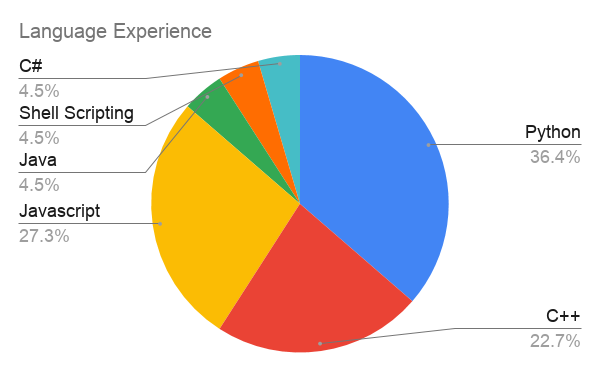
\includegraphics[width=\textwidth]{images/lang-experience.png}
  \label{fig:lang-experience}
\end{figure}

\begin{table}[htbp!]
\centering
\small
\caption{Backend Technology Decision Matrix}
\label{my-label}
\begin{spacing}{1.1}
\resizebox{\textwidth}{!}{
\begin{tabular}{@{}r c|c|c|c|c|c|c|c|c@{}}
\hline
\toprule

&
&\multicolumn{4}{c|}{\bfseries\footnotesize Python}
&\multicolumn{4}{c}{\bfseries\footnotesize Javascript}\\ \hline

\bfseries{\footnotesize Criteria} 
&\bfseries{\footnotesize Weight} 
&\multicolumn{2}{c|}{\bfseries\footnotesize Flask}
&\multicolumn{2}{c|}{\bfseries\footnotesize Django}
&\multicolumn{2}{c|}{\bfseries\footnotesize Express.js}
&\multicolumn{2}{c}{\bfseries\footnotesize Node.js}\\ \hline

     &  & {\footnotesize Score}&
     {\footnotesize Total}&
     {\footnotesize Score}&
     {\footnotesize Total}&
     {\footnotesize Score}&
     {\footnotesize Total}&
     {\footnotesize Score}&
     {\footnotesize Total}   \\\hline


Ease of Use     & 6 & 6 & 36 & 6 & 36 & 4 & 24 & 4 & 24   \\
DT Experience   & 6 & 6 & 36 & 6 & 36 & 4 & 24 & 4 & 24   \\
Simplicity      & 5 & 4 & 20 & 5 & 25 & 5 & 25 & 5 & 25   \\
Size            & 4 & 6 & 24 & 4 & 16 & 6 & 24 & 5 & 20   \\
Compatability*      & 6 & 6 & 36 & 5 & 30 & 6 & 36 & 6 & 36   \\ \hline
& Total &\multicolumn{2}{c|}{\bfseries\footnotesize 152}& \multicolumn{2}{c|}{\bfseries\footnotesize 143} &  \multicolumn{2}{c|}{\bfseries\footnotesize 133} &  \multicolumn{2}{c}{\bfseries\footnotesize 129}   \\

\bottomrule
\end{tabular}}
\end{spacing}{}
\end{table}

\subsection{Coding Standards}
Although Propic does not require the adoption of any specific technology or standard, the development team agreed that it would be good practice to still enforce coding standards to optimise consistency, readability and maintainability. Given the tech stack decisions, this was predominantly relevant to Python code (back-end) and JavaScript code (front-end). For these, the PEP style guidelines will be used for python with a small addition for function commenting (available on the project wiki) as well as the Airbnb JavaScript style guide which will be assisted with static analysis by ESLint.

\subsection{Integrated Development Environment}
\paragraph{Technologies Considered:}
VSCode, PyCharm, Jupiter Notebook, Vim, Atom, Sublime
\paragraph{Decision Criteria:}
\begin{itemize}
\item Compatibility for languages and frameworks to be used
\item Static analysis extensions (specifically for PEP and Airbnb style guides)
\item Development team experience and preference
\item Version control integration
\end{itemize}

\paragraph{Chosen:}
VSCode (preferred guideline)

\paragraph{Justification:}
Given the above decisions on languages, frameworks and coding standards, it was decided that the preferred IDE for development will be VSCode. This is because it is free, straightforward to use and has good support for Python as well as JavaScript in terms of syntax highlighting and extensions for static analysis. It is also extremely versatile with a rich library of extensions which make it highly customisable. The universal use of a VSCode throughout the team is not being mandated as a range of other IDEs can also be configured in accordance with the projects' style preferences. This allows any developer to use their own favourite IDE, if preferred.
\end{spacing}